
\section{HÌNH CHÓP TAM GIÁC ĐỀU, HÌNH CHÓP TỨ GIÁC ĐỀU}

\subsubsection{Kiến thức trọng tâm}

\begin{tcolorbox}[colback=gray!5, colframe=teal!60!black, boxrule=1pt, arc=7pt]
	\textbf{Hình chóp tam giác đều}
	\begin{tomtat}
	\immini{Hình $S.ABC$ (Hình bên) là một \textit{hình chóp tam giác đều}.\\
	Trong hình này:
	\begin{itemize}
		\item $S$ gọi là \textit{đỉnh}.
		\item Mặt $ABC$ là một tam giác đều và được gọi là \textit{mặt đáy} (gọi tắt là \textit{đáy}).
		\item Các đoạn thẳng $SA$, $SB$, $SC$ bằng nhau và được gọi là các \textit{cạnh bên}.
		\item Ba mặt $SAB$, $SBC$, $SCA$ là các tam giác cân bằng nhau và được gọi là \textit{ba mặt bên}.
		\item Các đoạn thẳng $AB$, $BC$, $CA$ được gọi là \textit{cạnh đáy}.
		\item Gọi $O$ là trọng tâm của mặt đáy, khi đó $SO$ gọi là \textit{đường cao}, độ dài $SO$ gọi là \textit{chiều cao}.
	\end{itemize}
}{
	\begin{tikzpicture}[font=\footnotesize, scale=1.2, line join =round, line cap= round, >= stealth,
	declare function={goc=-45; a=4.5; b=0.45*a; h=3.5;}]
	\path 
	(0,0) coordinate (A)
	(a,0) coordinate (C)
	(goc:b) coordinate (B)
	($(A)!.5!(C)$)coordinate (M)
	($(B)!.5!(C)$)coordinate (N)
	(intersection of B--M and A--N) coordinate (O)
	($(O)+(90:h)$) coordinate (S)
	;
	\fill[gray!15] (A)--(B)--(C)--cycle;
	\draw (S)--(A)--(B)--(C)--(S)--(B);
	\draw[dashed] (A)--(C) (B)--(M) (A)--(N) (S)--(O);
	\foreach \x/\g in {A/180,B/-90,C/0,S/120,O/-60}{
		\fill (\x) circle (1pt) node[shift={(\g:7pt)}] {$\x$};
	}	
	\draw pic[draw, angle radius=2mm]{right angle=S--O--A};
	\draw pic[draw, angle radius=2mm]{right angle=B--M--C};
	\draw pic[draw, angle radius=2mm]{right angle=A--N--B};
	\end{tikzpicture}
}
\end{tomtat}
\end{tcolorbox}


\begin{tcolorbox}[colback=gray!5, colframe=teal!60!black, boxrule=1pt, arc=7pt]
	\textbf{Hình chóp tứ giác đều}
	\begin{tomtat}
	\immini{Hình $S.ABCD$ (Hình bên) là một hình chóp tứ giác đều.\\
	Trong hình này:
	\begin{itemize}
		\item $S$ gọi là \textit{đỉnh}.
		\item Mặt $ABCD$ là một hình vuông và được gọi là \textit{mặt đáy} (gọi tắt là \textit{đáy}).
		\item Các đoạn thẳng $SA$, $SB$, $SC$, $SD$ bằng nhau và được gọi là các c\textit{ạnh bên}.
		\item Bốn mặt $SAB$, $SBC$, $SCD$, $SDA$ là các tam giác cân bằng nhau và được gọi là bốn \textit{mặt bên}.
		\item Các đoạn thẳng $AB$, $BC$, $CD$, $DA$ được gọi là \textit{cạnh đáy}.
		\item Gọi $O$ là giao điểm hai đường chéo của \textit{mặt đáy}, khi đó $SO$ là \textit{đường cao}, độ dài $SO$ là \textit{chiều cao}.
	\end{itemize}
}{
	\begin{tikzpicture}[font=\footnotesize, scale=1, line join =round, line cap= round, >= stealth,
	declare function={goc=-145; a=4; b=0.45*a; h=3.5;}]
	\path 
	(0,0) coordinate (A)
	(a,0) coordinate (D)
	(goc:b) coordinate (B)
	($(B)+(D)-(A)$) coordinate (C)
	($(A)!.5!(C)$)coordinate (O)
	($(O)+(90:h)$) coordinate (S)
	;
	\fill[gray!15] (A)--(B)--(C)--(D)--cycle;
	\draw (S)--(B)--(C)--(D)--(S)--(C)
	pic[angle radius=2mm]{right angle=S--O--A};
	\draw[dashed] (S)--(A)--(B) (A)--(D) (A)--(C) (B)--(D)
	(S)--(O);
	\foreach \x/\g in {A/160,B/-90,D/0,S/120,C/-60,O/-90}{
		\fill (\x) circle (1pt) node[shift={(\g:7pt)}] {$\x$};
	}
\draw pic[draw, angle radius=2mm]{right angle=S--O--A};
	\end{tikzpicture}
}
\end{tomtat}
\end{tcolorbox}
\newpage


\begin{vd}%[Dự án EX-9-Đề Cương Toán 9]%[Lương Pho, TVN-541]%[8H1N1-1]
	\immini{Hãy cho biết cạnh bên, mặt bên, cạnh đáy, mặt đáy, đường cao, độ dài cạnh bên, độ dài cạnh đáy của hình chóp tam giác đều ở hình bên.
	}{
	\begin{tikzpicture}[font=\footnotesize, scale=1, line join =round, line cap= round, >= stealth,
	declare function={goc=-45; a=4.5; b=0.45*a; h=3.5;}]
	\path 
	(0,0) coordinate (A)
	(a,0) coordinate (C)
	(goc:b) coordinate (B)
	($(A)!.5!(C)$)coordinate (M)
	($(B)!.5!(C)$)coordinate (N)
	(intersection of B--M and A--N) coordinate (O)
	($(O)+(90:h)$) coordinate (S)
	;
	\draw (S)--(A)--(B)--(C)--(S)--(B);
	\draw[dashed] (A)--(C) (B)--(M) (A)--(N) (S)--(O);
	\foreach \x/\g in {A/180,B/-90,C/0,S/120,O/-60}{
		\fill (\x) circle (1pt) node[shift={(\g:7pt)}] {$\x$};
	}
	\path (B)--(C) node[pos=.5, below,sloped] {$12$ cm};
	\path (S)--(A) node[pos=.5, above,sloped] {$8$ cm};
%	\path (S)--(O) node[pos=.5, above,sloped] {$4$ cm};

\draw pic[draw, angle radius=2mm]{right angle=S--O--A};
	\end{tikzpicture}
}
\loigiai{
	Hình chóp tam giác đều $S.ABC$, có
\begin{itemize}
	\item Cạnh đáy là $AB$, $BC$, $CA$ và có độ dài bằng $12$ cm.
	\item Cạnh bên là $SA$, $SB$, $SC$ và có độ dài bằng $8$ cm.
	\item Đường cao là cạnh $SO$.
	\item Mặt bên là các mặt $SAB$, $SAC$, $SBC$.
	\item Mặt đáy là mặt $ABC$.
\end{itemize}
}
\end{vd}

\begin{vd}%[Dự án EX-9-Đề Cương Toán 9]%[Lương Pho, TVN-541]%[8H1H1-2]
	Tạo lập hình chóp tứ giác đều có độ dài cạnh đáy $6$ cm và cạnh bên $8$ cm theo hướng dẫn sau:
	\begin{itemize}
		\item Trên một tấm bìa, vẽ một hình vuông và bốn hình tam giác cân với kích thước như Hình a.
		\item Cắt tấm bìa như hình vẽ, rồi gấp theo các đường màu đỏ ta được hình chóp tứ giác đều như Hình b.
	\end{itemize}
\begin{center}
	\begin{tabular}{cc}
	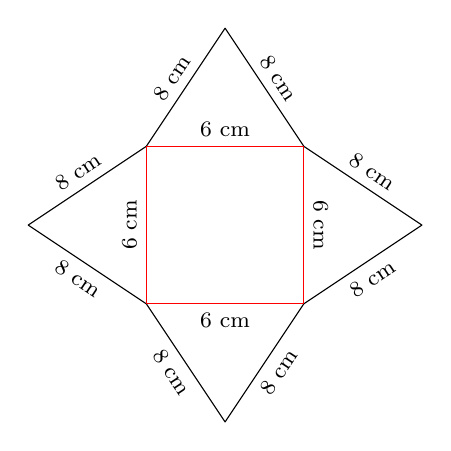
\begin{tikzpicture}[font=\footnotesize, scale=1, line join =round, line cap= round, >= stealth,
	declare function={a=1; b=2.5;}]
	\path 
	(-b,0) coordinate (M)
	(0,b) coordinate (N)
	(b,0) coordinate (P)
	(0,-b) coordinate (Q)
	(-a,a) coordinate (A)
	(a,a) coordinate (B)
	(a,-a) coordinate (C)
	(-a,-a) coordinate (D)
	;
	\draw (-b,0)--(-a,a)--(0,b)--(a,a)--(b,0)--(a,-a)--(0,-b)--(-a,-a)--cycle;
	\draw[red] (a,a) rectangle (-a,-a);
	\foreach \a/\b/\vitri/\nhan in {M/A/above/8,A/N/above/8,N/B/above/8,B/P/above/8,P/C/below/8,C/Q/below/8,Q/D/below/8,D/M/below/8,A/B/above/6,B/C/above/6,C/D/below/6,D/A/above/6}{
	\path (\a)--(\b) node[midway, sloped, \vitri]{$\nhan$ cm};
}
	\end{tikzpicture}
	&
	\begin{tikzpicture}[font=\footnotesize, scale=1, line join =round, line cap= round, >= stealth,
	declare function={goc=-145; a=4; b=0.45*a; h=3.5;}]
	\path 
	(0,0) coordinate (A)
	(a,0) coordinate (D)
	(goc:b) coordinate (B)
	($(B)+(D)-(A)$) coordinate (C)
	($(A)!.5!(C)$)coordinate (O)
	($(O)+(90:h)$) coordinate (S)
	;
	\draw (S)--(B)--(C)--(D)--(S)--(C);
	\draw[dashed] (S)--(A)--(B) (A)--(D) ;
	%	(S)--(O);
%	\foreach \x/\g in {A/160,B/-90,D/0,S/120,C/-60}{
%		\fill (\x) circle (1pt) node[shift={(\g:7pt)}] {$\x$};
%	}
	\end{tikzpicture}\\
	Hình a&Hình b
\end{tabular}
\end{center}
\end{vd}

\begin{vd}%[Dự án EX-9-Đề Cương Toán 9]%[Lương Pho, TVN-541]%[8H1H1-1]
	\immini{Cho hình chóp tứ giác đều $S.ABCD$ như hình vẽ bên. Cho biết $SA=6$ cm, $CD=5$ cm. Tìm độ dài các cạnh $SB$, $SC$, $SD$, $AB$, $BC$, $AD$.
	}{
	\begin{tikzpicture}[font=\footnotesize, scale=1, line join =round, line cap= round, >= stealth,
	declare function={goc=-145; a=3.2; b=0.45*a; h=2.8;}]
	\path 
	(0,0) coordinate (A)
	(a,0) coordinate (D)
	(goc:b) coordinate (B)
	($(B)+(D)-(A)$) coordinate (C)
	($(A)!.5!(C)$)coordinate (O)
	($(O)+(90:h)$) coordinate (S)
	;
	\draw (S)--(B)--(C)--(D)--(S)--(C)
	pic[angle radius=2mm]{right angle=S--O--A};
	\draw[dashed] (S)--(A)--(B) (A)--(D) (A)--(C) (B)--(D)
	(S)--(O);
	\foreach \x/\g in {A/160,B/-90,D/0,S/120,C/-60,O/-90}{
		\fill (\x) circle (1pt) node[shift={(\g:7pt)}] {$\x$};
	}
	\end{tikzpicture}
}
	\loigiai{
		Vì $S.ABCD$ là hình chóp tứ giác đều, nên
		\begin{itemize}
			\item Các cạnh bên bằng nhau $SA=SB=SC=SD=6$ cm.
			\item Mặt đáy $ABCD$ là hình vuông nên các cạnh đáy bằng nhau $AB=BC=CD=DA=5$ cm.
	\end{itemize}
}
\end{vd}

\begin{vd}%[Dự án EX-9-Đề Cương Toán 9]%[Lương Pho, TVN-541]%[8H1H1-2]
	Chiếc hộp được vẽ lại như bên dưới có dạng hình chóp tam giác đều $S.MNP$. Cho biết $SM=5$ cm, $MN=4$ cm.
	\begin{center}
		\begin{tikzpicture}[font=\footnotesize, scale=1, line join =round, line cap= round, >= stealth,
		declare function={goc=25; a=4; b=0.5*a; h=2.8;}]
		\path 
		(0,0) coordinate (A)
		(5:a) coordinate (B)
		(goc:b) coordinate (C)
		($(C)+(85:h)$) coordinate (S)
		;
		\fill[teal!70] (S)--(A)--(C)--(B)--(S)--(C)--cycle;
		\fill[gray!70] (A)--(B)--(C)--cycle;
		\draw[teal!60!white, line width=3pt] (S)--(A)--(C)--(B)--(S)--(C)--cycle;
		\draw[gray!60!white, line width=3pt] (A)--(B);
		\end{tikzpicture}
		\qquad
		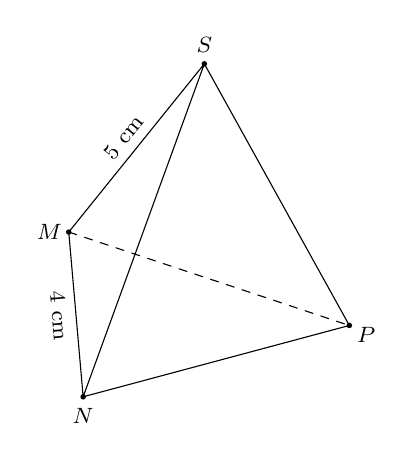
\begin{tikzpicture}[font=\footnotesize, scale=1, line join =round, line cap= round, >= stealth,
		declare function={goc=15; a=3.5; b=0.6*a; h=4.5;}]
		\path 
		(0,0) coordinate (N)
		(goc:a) coordinate (P)
		(95:b) coordinate (M)
		(70:h) coordinate (S)
		;
		\draw (S)--(M)--(N)--(P)--(S)--(N);
		\draw[dashed](M)--(P);
		\foreach \x/\g in {N/-90,P/-30,M/180,S/90}{
			\fill (\x) circle (1pt) node[shift={(\g:7pt)}] {$\x$};
		}
		\path (M)--(N) node[pos=.5, below,sloped] {$4$ cm};
		\path (S)--(M) node[pos=.5, above,sloped] {$5$ cm};
		\end{tikzpicture}
	\end{center}
	\begin{enumerate}
		\item Tìm độ dài các cạnh còn lại của chiếc hộp.
		\item Mỗi góc của tam giác đáy $MNP$ bằng bao nhiêu độ?
	\end{enumerate}
	\loigiai{
	\begin{enumerate}
			\item Vì $S.MNP$ là hình chóp tam giác đều nên
		\begin{itemize}
			\item Các cạnh bên bằng nhau $SN=SP=SM=5$ cm.
			\item Mặt đáy $MNP$ là tam giác đều nên các cạnh đáy bằng nhau $NP=PM=MN=4$ cm.
		\end{itemize}	
		\item Vì tam giác đáy $MNP$ là tam giác đều nên mỗi góc của tam giác đều bằng $60^\circ$.\\
		Vậy $\widehat{M}=\widehat{N}=\widehat{P}=60^\circ$.
	\end{enumerate}
	}
\end{vd}

\subsubsection{Bài tập}
\begin{bt}%[Dự án EX-9-Đề Cương Toán 9]%[Lương Pho, TVN-541]%[8H1H1-1]
		Quan sát hình vẽ dưới đây và thay mỗi dấu ? cho thích hợp.
		\begin{center}
			\renewcommand{\arraystretch}{1.6} % tăng độ cao hàng
			\begin{tabular}{|c|c|c|c|c|c|}
				\hline
				\textbf{Hình} & \textbf{Đáy} & \textbf{Mặt bên} & \textbf{Số cạnh đáy} & \textbf{Số cạnh bên} & \textbf{Số mặt} \\
				\hline
				\begin{tabular}{c}
					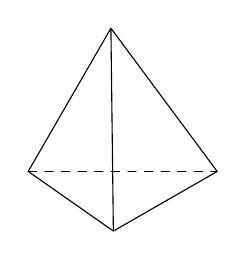
\begin{tikzpicture}[font=\footnotesize, scale=.6, line join =round, line cap= round, >= stealth,
					declare function={goc=-35; a=4; b=0.55*a; h=3.5;}]
					\path 
					(0,0) coordinate (A)
					(60:h) coordinate (S)
					(a,0) coordinate (C)
					(goc:b) coordinate (B);
					\draw (S)--(A)--(B)--(C)--(S)--(B);
					\draw[dashed] (A)--(C);
					\end{tikzpicture}\\
					\textbf{Hình chóp tam giác đều}
				\end{tabular}
				& ? & Tam giác cân & ? & ? & ? \\
				\hline
				\begin{tabular}{c}
					\begin{tikzpicture}[font=\footnotesize, scale=.6, line join =round, line cap= round, >= stealth,
					declare function={goc=-35; a=4; b=0.55*a; h=3.5;}]
					\path 
					(0,0) coordinate (A)
					(60:h) coordinate (S)
					(a,0) coordinate (C)
					(goc:b) coordinate (B)
					($(A)+(C)-(B)$) coordinate (D);
					\draw (S)--(A)--(B)--(C)--(S)--(B);
					\draw[dashed] (A)--(D)--(C) (S)--(D);
					\end{tikzpicture}\\
					\textbf{Hình chóp tứ giác đều}
				\end{tabular}
				& Hình vuông & ?& ? & ? & ? \\
				\hline
			\end{tabular}
		\end{center}
	\loigiai{
	Ta có bảng đầy đủ sau:
	\begin{center}
		\renewcommand{\arraystretch}{1.8} % tăng độ cao hàng
		\begin{tabular}{|c|c|c|c|c|c|}
			\hline
			\textbf{Hình} & \textbf{Đáy} & \textbf{Mặt bên} & \textbf{Số cạnh đáy} & \textbf{Số cạnh bên} & \textbf{Số mặt} \\
			\hline
			\begin{tabular}{c}
				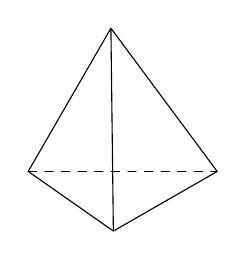
\begin{tikzpicture}[font=\footnotesize, scale=.6, line join =round, line cap= round, >= stealth,
				declare function={goc=-35; a=4; b=0.55*a; h=3.5;}]
				\path 
				(0,0) coordinate (A)
				(60:h) coordinate (S)
				(a,0) coordinate (C)
				(goc:b) coordinate (B);
				\draw (S)--(A)--(B)--(C)--(S)--(B);
				\draw[dashed] (A)--(C);
				\end{tikzpicture}\\
				\textbf{Hình chóp tam giác đều}
			\end{tabular}
			& Tam giác đều & Tam giác cân & $3$ & $3$ & $4$ \\
			\hline
			\begin{tabular}{c}
				\begin{tikzpicture}[font=\footnotesize, scale=.6, line join =round, line cap= round, >= stealth,
				declare function={goc=-35; a=4; b=0.55*a; h=3.5;}]
				\path 
				(0,0) coordinate (A)
				(60:h) coordinate (S)
				(a,0) coordinate (C)
				(goc:b) coordinate (B)
				($(A)+(C)-(B)$) coordinate (D);
				\draw (S)--(A)--(B)--(C)--(S)--(B);
				\draw[dashed] (A)--(D)--(C) (S)--(D);
				\end{tikzpicture}\\
				\textbf{Hình chóp tứ giác đều}
			\end{tabular}
			& Hình vuông & Tam giác cân & $4$ & $4$ & $5$ \\
			\hline
		\end{tabular}
	\end{center}
	
}
\end{bt}
\begin{bt}%[Dự án EX-9-Đề Cương Toán 9]%[Lương Pho, TVN-541]%[8H1N1-1]
	\immini{Cho hình chóp tam giác đều $M.NPQ$ ở hình vẽ bên. Hãy xác định độ dài cạnh đáy, cạnh bên và đường cao của hình chóp đó.
	}{
		\begin{tikzpicture}[font=\footnotesize, scale=1, line join =round, line cap= round, >= stealth,
		declare function={goc=-45; a=4.5; b=0.45*a; h=3.5;}]
		\path 
		(0,0) coordinate (A)
		(a,0) coordinate (C)
		(goc:b) coordinate (B)
		($(A)!.5!(C)$)coordinate (M)
		($(B)!.5!(C)$)coordinate (N)
		(intersection of B--M and A--N) coordinate (O)
		($(O)+(90:h)$) coordinate (S)
		;
		\draw (S)--(A)--(B)--(C)--(S)--(B);
		\draw[dashed] (A)--(C) (B)--(M) (A)--(N) (S)--(O);
		\foreach \x/\g/\nhan in {A/180/N,B/-90/P,C/0/Q,S/120/M,O/-60/H}{
			\fill (\x) circle (1pt) node[shift={(\g:7pt)}] {$\nhan$};
		}
		\path (B)--(C) node[pos=.5, below,sloped] {$6$ cm};
		\path (S)--(A) node[pos=.5, above,sloped] {$4$ cm};
			\path (S)--(O) node[pos=.5, above,sloped] {$2$ cm};
		
		\draw pic[draw, angle radius=2mm]{right angle=S--O--A};
		\end{tikzpicture}
	}
	\loigiai{
		Hình chóp tam giác đều $M.NPQ$, có
		\begin{itemize}
			\item Độ dài cạnh đáy bằng $6$ cm.
			\item Độ dài cạnh bên bằng $4$ cm.
			\item Độ dài đường cao bằng $2$ cm.
		\end{itemize}
	}
\end{bt}

\begin{bt}%[Dự án EX-9-Đề Cương Toán 9]%[Lương Pho, TVN-541]%[8H1H1-1]
	\immini{Cho hình chóp tứ giác đều $K.MNPQ$ ở hình vẽ bên. Hãy xác định độ dài cạnh đáy, cạnh bên và chiều cao của hình chóp đó.
	}{
		\begin{tikzpicture}[font=\footnotesize, scale=1.2, line join =round, line cap= round, >= stealth,
		declare function={goc=-145; a=3.2; b=0.45*a; h=2.8;}]
		\path 
		(0,0) coordinate (A)
		(a,0) coordinate (D)
		(goc:b) coordinate (B)
		($(B)+(D)-(A)$) coordinate (C)
		($(A)!.5!(C)$)coordinate (O)
		($(O)+(90:h)$) coordinate (S)
		;
		\draw (S)--(B)--(C)--(D)--(S)--(C)
		pic[angle radius=2mm]{right angle=S--O--A};
		\draw[dashed] (S)--(A)--(B) (A)--(D) (A)--(C) (B)--(D)
		(S)--(O);
		\foreach \x/\g/\nhan in {A/160/M,B/-90/N,D/0/Q,S/120/K,C/-60/P,O/-90/H}{
			\fill (\x) circle (1pt) node[shift={(\g:7pt)}] {$\nhan$};
		}
		\path (B)--(C) node[pos=.5, below,sloped] {$8$ cm};
		\path (S)--(D) node[pos=.5, above,sloped] {$6$ cm};
		\path (S)--(O) node[pos=.5, below,sloped] {$2$ cm};
		\draw pic[draw, angle radius=2mm]{right angle=S--O--A};
		\end{tikzpicture}
	}
	\loigiai{
		Hình chóp tứ giác đều $K.MNPQ$, có
		\begin{itemize}
			\item Độ dài cạnh đáy bằng $8$ cm.
			\item Độ dài cạnh bên bằng $6$ cm.
			\item Chiều cao bằng $2$ cm.
		\end{itemize}
	}
\end{bt}
\begin{bt}%[Dự án EX-9-Đề Cương Toán 9]%[Lương Pho, TVN-541]%[8H1H1-3]
	Một Kim tự tháp Kheops - Ai Cập (hình bên trái) có dạng hình chóp tứ giác đều, đáy là hình vuông, các mặt bên là các tam giác cân chung đỉnh (hình minh họa bên phải). Với các kích thước được cho ở hình vẽ, hãy cho biết chiều cao và cạnh đáy bằng bao nhiêu mét?
	\begin{center}
		\begin{tabular}{c c}			
			\begin{tikzpicture}[line join = round, line cap=round,>=stealth,font=\footnotesize,scale=1]		
			\fill[pattern=bricks, pattern color=gray](0,0)--(3,-0.5)--(3.5,4)--cycle 	;
			\fill[pattern=bricks] (3,-0.5)--(3.5,4)--(7,0)--cycle 	;
			\draw 	(0,0)--(3,-0.5)--(7,0) --(3.5,4)--cycle 	(3,-0.5)--(3.5,4)	;	
			\end{tikzpicture} & \begin{tikzpicture}[font=\footnotesize, line join=round, line cap=round, >=stealth]
			\path
			(0,0) coordinate (A)
			(4,0) coordinate (B)
			(-2,-1) coordinate (D)
			($(B)+(D)-(A)$) coordinate (C)
			($(A)!.5!(C)$) coordinate (O)
			($(O)+(0,3.5)$) coordinate (S)
			;
			\draw (S)--(D)--(C)node[midway,below]{$240$ m}--(S)--(B)--(C);
			\draw[dashed] (B)--(D)--(A)--(S)--(O)node[midway,above right,sloped]{$140$ m} (B)--(A)--(C);
			\foreach \x/\y/\z in {S/O/B} {
				\path 
				($(\y)!5pt!(\z)$) coordinate (1)
				($(\y)!5pt!(\x)$) coordinate (2)
				($(1)+(2)-(\y)$) coordinate (3)
				;
				\draw (1)--(3)--(2);
			}
			\foreach \x/\y in {A/135,B/45,C/-45,D/-135,O/-90,S/90}
			\fill(\x) circle (0.3mm) + (\y:0.3) node {$\x$};
			\end{tikzpicture} \\ 
		\end{tabular} 
	\end{center}
	\loigiai{
		Chiều cao của kim tự tháp khoảng $140$ mét, cạnh đáy của nó dài $240$ mét.		
	}
\end{bt}

\begin{bt}%[Dự án EX-9-Đề Cương Toán 9]%[Lương Pho, TVN-541]%[8H1H1-3]
	Hình chóp được đặt trên đỉnh Fansipan là một hình chóp tam giác đều được làm bằng inox. Hình chóp có cạnh đáy bằng $60$\,cm, các mặt bên là tam giác cân có cạnh bên dài $1$ mét. Biết rằng chỉ có các mặt bên của hình chóp mới được làm bằng inox. Hình chóp được minh họa như \textit{hình 2}. Hãy cho biết độ dài $AB$, $BC$, $AC$, $SA$, $SB$, $SC$?\\
	\begin{minipage}{0.45\textwidth} 
		\centering 
		
\begin{tikzpicture}[line join = round, line cap=round,>=stealth,font=\footnotesize,scale=1.2]
		%%%%%%%%%%%%%%%
		\draw[fill=black!10] 
		(-1.30,-1.00) -- (0.70,4.00) -- (1.30,-1.00)--cycle
		(0.70,4.00) -- (2.50,-1.00)--(1.30,-1.00) --cycle;
		\draw[fill=orange]  
		(2.20,-0.15)--(2.50,-1.00)--(1.30,-1.00)--(1.25,-0.55)--cycle
		(1.30,-1.00)--(1.25,-0.55)--(-0.95,-0.10) --(-1.30,-1.00)--cycle;
		%%%%%%%%%%%%%%%
		\draw[fill=black] (-0.33,1.20) ..controls +(75:0.6) and +(95:1.1) .. (0.83,1.2)
		..controls +(-90:1.2) and +(-105:1.45) ..cycle;
		%%%%%%%%%%%%%%%
		\draw[fill=white] (-0.25,1.20)..controls +(65:0.7) and +(95:0.85) ..(0.75,1.2)
		..controls +(-85:0.9) and +(-105:1.53) ..(-0.25,1.20);
		%%%%%%%%%%%%%%%
		\draw[fill=black!91,opacity=0.1,xshift=3pt] (-0.30,1.20) -- (0.00,1.21) -- (0.19,1.67) -- (0.26,1.27) -- (0.61,1.29) -- (0.26,0.97) -- (0.29,0.51) -- (0.04,0.76) -- (-0.26,0.51) -- (-0.11,0.96)--cycle;
		\draw[fill=orange] (-0.30,1.20) -- (0.00,1.21) -- (0.19,1.67) -- (0.26,1.27) -- (0.61,1.29) -- (0.26,0.97) -- (0.29,0.51) -- (0.04,0.76) -- (-0.26,0.51) -- (-0.11,0.96)--cycle;
		\draw[white] (-0.02,1.05)--(-0.30,1.20)(-0.02,1.05)--(0.19,1.67)(-0.02,1.05)--(0.61,1.29)(-0.02,1.05)--(0.29,0.51)(-0.02,1.05)--(-0.26,0.51);
		\draw[fill=black] (1.15,1.25) ..controls +(95:0.8) and +(110:1).. (1.78,1.05)
		..controls +(-75:1.3) and +(-85:1).. cycle;
		\draw[fill=white] (1.25,1.25) ..controls +(100:0.65) and +(110:1).. (1.78,1.05)
		..controls +(-76:1.1) and +(-85:0.95).. cycle;
		\draw[fill=orange] 
		(1.75,1.05) -- (1.40,1.75) -- (1.45,1.30) -- (1.30,1.25) -- (1.50,0.95) -- (1.57,0.45) -- (1.70,0.70) -- (1.80,0.50)--cycle
		;
		\draw[white](1.73,1.05)--(1.41,1.7)(1.73,1.05)--(1.30,1.25)(1.73,1.05)--(1.57,0.45)(1.73,1.05)--(1.80,0.50);
		\end{tikzpicture}
		\\
		Hình 1 
	\end{minipage}
	\hfill 
	\begin{minipage}{0.45\textwidth}
		\centering
		\begin{tikzpicture}[line join = round, line cap=round,>=stealth,font=\footnotesize,scale=1]
		\path 
		(0,0) coordinate (A)
		(0:5) coordinate (B)
		(-30:4) coordinate (C)
		($(B)!.5!(C)$) coordinate (E)
		($(A)!2/3!(E)$) coordinate (O)
		($(O)+(0,5)$) coordinate (S)			
		;
		\draw(S)--(C)--(B)--(S)--(A)--(C);
		\draw[dashed]  (B)--(A);
		\foreach \x/\g in {A/210,B/-30,C/-60,S/90} \fill (\x) circle (1pt) +(\g:3mm) node{$\x$};
		\end{tikzpicture}
		\\
		Hình 2
	\end{minipage}
	\loigiai{
		Vì $S.ABC$ là hình chóp tam giác đều nên
		\begin{itemize}
			\item Các cạnh bên bằng nhau $SA=SB=SC=1$ m.
			\item Mặt đáy $ABC$ là tam giác đều nên các cạnh đáy bằng nhau $AB=BC=CA=60$ cm.
		\end{itemize}	
	}
\end{bt}
\begin{bt}%[Dự án EX-9-Đề Cương Toán 9]%[Lương Pho, TVN-541]%[8H1H1-3]
	\immini{Một mái che giếng trời làm bằng kính có dạng hình chóp tứ giác đều với độ dài cạnh đáy là $2{,}2$ m và chiều cao từ mặt đáy tới đỉnh của hình chóp tứ giác đều là $2{,}6$ m. Tính diện tích mặt đáy giếng trời.
}{
		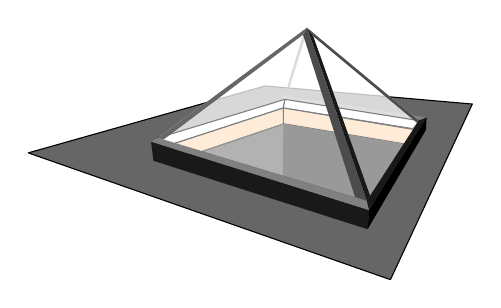
\begin{tikzpicture}[line join = round, line cap=round,>=stealth,font=\footnotesize,scale=1]
		%Nền sân
		\draw [fill=black!60](-3.51,-0.66) -- (-0.5,0.19) -- (2.13,-0.04) -- (1.09,-2.27)--cycle;
		%Cạnh sau
		\fill[black!60](0.03,0.93)--(-0.25,0.02)--(-0.27,0.01) -- (-0.02,0.84)--cycle;
		\fill[black!60](0.03,0.93)--(-0.25,0.02)--(-0.24,0.02) -- (0.02,0.85)--cycle;
		%Chân sau trái
		\fill[black!50](-0.26,-0.01) -- (-0.28,0.01) -- (-1.86,-0.47)-- (-1.95,-0.52)--cycle;
		%Chân sau phải
		\fill[black!50](-0.28,0.07) -- (-0.27,0.01) -- (1.45,-0.25)-- (1.55,-0.21)--cycle;
		%Mặt sau trái
		\fill[white,opacity=0.5](0.03,0.93) -- (-0.25,0.02) -- (-1.86,-0.47)--cycle;
		%Mặt sau phải
		\fill[white,opacity=0.5](0.03,0.93) -- (-0.25,0.02) -- (1.45,-0.25)--cycle;
		%Tường trong
		\draw[fill=white!40](-1.86,-0.47)--(-0.25,0.02)--(-0.27,-0.09) -- (-1.65,-0.54);
		\draw[fill=white!40](1.45,-0.25)--(-0.25,0.02)--(-0.27,-0.09)--(1.36,-0.35);
		\draw[fill=orange!30](-0.27,-0.09) -- (-1.65,-0.54) -- (-1.68,-0.77)--(-0.26,-0.29)--cycle;
		\draw[black!80](-0.27,-1) -- (-1.53,-0.85) -- (-1.68,-0.77)--(-0.26,-0.29)--cycle;
		\draw[fill=orange!30](-0.27,-0.09)--(-0.27,-0.29)--(1.35,-0.56)--(1.43,-0.37)--cycle;
		\fill[black!80](-0.27,-1.09)--(-0.27,-0.29)--(1.35,-0.56)--(0.93,-1.31)--cycle;
		%Mặt trước trái
		\fill[white,opacity=0.5](0.03,0.93) -- (0.79,-1.27) -- (-1.86,-0.47)--cycle;
		%Mặt trước phải
		\fill[white,opacity=0.5](0.03,0.93) -- (0.79,-1.27) -- (1.45,-0.25)--cycle;
		%Cạnh trước
		\fill[black!90](0.03,0.93)--(0.79,-1.27)--(0.83,-1.2) -- (0.11,0.82)--cycle;
		\fill[black!70](0.03,0.93)--(0.79,-1.27)--(0.64,-1.22) -- (-0.02,0.84)--cycle;
		%Cạnh phải
		\fill[black!70](0.03,0.93)--(1.45,-0.25)--(1.43,-0.28) -- (0.11,0.82)--cycle;
		%Cạnh trái
		\fill[black!60](0.03,0.93)--(-1.86,-0.47)--(-1.79,-0.49) -- (-0.02,0.84)--cycle;
		%Chân trước trái
		\fill[black!50](0.82,-1.39) -- (0.79,-1.27) -- (-1.86,-0.47)-- (-1.95,-0.52)--cycle;
		\fill[black!90](0.82,-1.39) -- (0.8,-1.63) -- (-1.92,-0.76)-- (-1.95,-0.52)--cycle;
		%Chân trước phải
		\fill[black!90](0.82,-1.39) -- (0.79,-1.27) -- (1.45,-0.25)-- (1.55,-0.21)--cycle;
		\fill[black!100](0.82,-1.39) -- (0.8,-1.63) -- (1.54,-0.37)-- (1.55,-0.21)--cycle;
		\end{tikzpicture}
}
	\loigiai{
		Giếng trời có dạng hình chóp tứ giác đều nên đáy là hình vuông cạnh bằng $2{,}2$ m.\\
		Vậy diện tích mặt đáy của giếng trời bằng $2{,}2\cdot 2{,}2=4{,}48$ m$^2$.
	}
\end{bt}

\begin{bt}%[Dự án EX-9-Đề Cương Toán 9]%[Lương Pho, TVN-541]%[8H1H1-3]
	Chị Minh cần gấp một cái hộp quà có dạng hình chóp tứ giác đều từ tấm bài (hình bên dưới).
	Hộp quà tạo thành khi gấp có cạnh đáy và cạnh bên bằng bao nhiêu cm?
	\begin{center}
		\begin{tabular}{cc}
			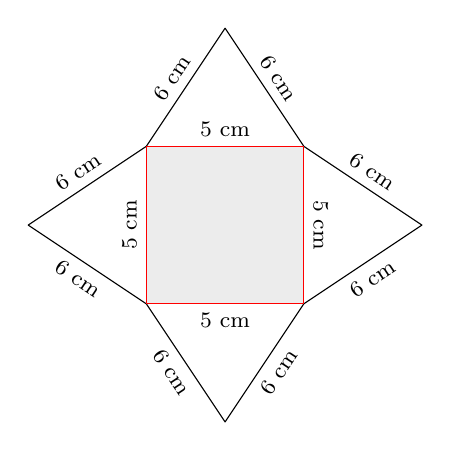
\begin{tikzpicture}[font=\footnotesize, scale=1, line join =round, line cap= round, >= stealth,
			declare function={a=1; b=2.5;}]
			\path 
			(-b,0) coordinate (M)
			(0,b) coordinate (N)
			(b,0) coordinate (P)
			(0,-b) coordinate (Q)
			(-a,a) coordinate (A)
			(a,a) coordinate (B)
			(a,-a) coordinate (C)
			(-a,-a) coordinate (D)
			;
			\draw (-b,0)--(-a,a)--(0,b)--(a,a)--(b,0)--(a,-a)--(0,-b)--(-a,-a)--cycle;
			\fill[gray!15] (a,a) rectangle (-a,-a);
			\draw[red] (a,a) rectangle (-a,-a);
			
			\foreach \a/\b/\vitri/\nhan in {M/A/above/6,A/N/above/6,N/B/above/6,B/P/above/6,P/C/below/6,C/Q/below/6,Q/D/below/6,D/M/below/6,A/B/above/5,B/C/above/5,C/D/below/5,D/A/above/5}{
				\path (\a)--(\b) node[midway, sloped, \vitri]{$\nhan$ cm};
			}
			\end{tikzpicture}
			&
			\begin{tikzpicture}[font=\footnotesize, scale=1, line join =round, line cap= round, >= stealth,
			declare function={goc=-145; a=4; b=0.45*a; h=3.5;}]
			\path 
			(0,0) coordinate (A)
			(a,0) coordinate (D)
			(goc:b) coordinate (B)
			($(B)+(D)-(A)$) coordinate (C)
			($(A)!.5!(C)$)coordinate (O)
			($(O)+(90:h)$) coordinate (S)
			;
			\fill[gray!15] (A)--(B)--(C)--(D)--cycle;
			\draw (S)--(B)--(C)--(D)--(S)--(C);
			\draw[dashed] (S)--(A)--(B) (A)--(D) ;
			%	(S)--(O);
			%	\foreach \x/\g in {A/160,B/-90,D/0,S/120,C/-60}{
			%		\fill (\x) circle (1pt) node[shift={(\g:7pt)}] {$\x$};
			%	}
			\end{tikzpicture}\\
			Tấm bìa cần gấp &Hộp quà tạo thành
		\end{tabular}
	\end{center}
\loigiai{
	Hộp quà tạo thành khi gấp có cạnh đáy bằng $5$ cm và cạnh bên bằng $6$ cm.
}
\end{bt}
\begin{bt}%[Dự án EX-9-Đề Cương Toán 9]%[Lương Pho, TVN-541]%[8H1H1-2]
	\immini{Hộp quà được gấp từ tấm bìa hình bên tạo thành hình chóp gì? Hãy cho biết độ dài cạnh bên và cạnh đáy của hình chóp tạo thành đó.
	}{
	\begin{tikzpicture}[font=\footnotesize, scale=1, line join =round, line cap= round, >= stealth,
	declare function={a=2; b=4.3;}]
	\path 
	(0,0) coordinate (A)
	(a,0) coordinate (C)
	(60:a) coordinate (B)
	(30:b) coordinate (N)
	($(C)+(150:b)$) coordinate (M)
	($(B)+(-90:b)$) coordinate (P)
	;
	\draw (M)--(B)--(N)--(C)--(P)--(A)--cycle;
	\fill[gray!15] (A)--(B)--(C);
	\draw (A)--(B)--(C)--cycle;
	
	\foreach \a/\b/\vitri/\nhan in {M/B/above/5,B/N/above/5,N/C/below/5,C/P/below/5,P/A/below/5,A/M/below/5,A/B/above/4,B/C/above/4,C/A/below/4}{
		\path (\a)--(\b) node[midway, sloped, \vitri]{$\nhan$ cm};
	}
	\end{tikzpicture}
}
	\loigiai{
		\begin{center}
			\begin{tikzpicture}[font=\footnotesize, scale=1, line join =round, line cap= round, >= stealth,
		declare function={goc=-45; a=4.5; b=0.45*a; h=3.5;}]
		\path 
		(0,0) coordinate (A)
		(a,0) coordinate (C)
		(goc:b) coordinate (B)
		($(A)!.5!(C)$)coordinate (M)
		($(B)!.5!(C)$)coordinate (N)
		(intersection of B--M and A--N) coordinate (O)
		($(O)+(90:h)$) coordinate (S)
		;
		\fill[gray!15] (A)--(B)--(C);
		\draw (S)--(A)--(B)--(C)--(S)--(B);
		\draw[dashed] (A)--(C);
%		\foreach \x/\g/\nhan in {A/180/N,B/-90/P,C/0/Q,S/120/M,O/-60/H}{
%			\fill (\x) circle (1pt) node[shift={(\g:7pt)}] {$\nhan$};
%		}
		\path (B)--(C) node[pos=.5, below,sloped] {$4$ cm};
		\path (S)--(A) node[pos=.5, above,sloped] {$5$ cm};
		
		\end{tikzpicture}
		\end{center}
		Hộp quà được gấp từ tấm bìa hình bên tạo thành hình chóp tam giác đều có độ dài cạnh bên bằng $5$ cm; độ dài cạnh đáy bằng $4$ cm.
	}
\end{bt}

